%%%%%%%%%%%%%%%%%%%%%%%%%%%%%%%%%%%%%%%%%%%%%%%%%%%%%%%%%%%%%%%%%%%
% 
% $Id: sec6.tex,v 1.1.1.1 2002/01/02 19:36:28 phil Exp $
%
% $Log: sec6.tex,v $
% Revision 1.1.1.1  2002/01/02 19:36:28  phil
% initial import into CVS
%
% Revision 1.10  1997/08/29 20:06:12  allen
% *** empty log message ***
%
% Revision 1.9  1996/08/14 17:59:42  phil
% fixed \bf
%
% Revision 1.8  1996/08/13 00:56:12  cguo
% glossary a problem
%
% Revision 1.7  1996/08/12 23:32:25  cguo
% here is v1.5 back again
%
% Revision 1.5  1996/08/06 21:39:58  cguo
% *** empty log message ***
%
% Revision 1.4  1996/08/02 22:18:31  cguo
% break up problems into parts
%
% Revision 1.3  1996/04/29 19:03:40  stockie
% ready for carmen
%
% Revision 1.2  1995/08/14  22:23:35  stockie
% - replace pendulum example with weather balloon; add plots
% - add sections on BVP's and PDE's
%
% Revision 1.1  1995/07/18  21:39:20  stockie
% Initial revision
%
%
%%%%%%%%%%%%%%%%%%%%%%%%%%%%%%%%%%%%%%%%%%%%%%%%%%%%%%%%%%%%%%%%%%%

\section{Generalizations}

%%%%%%%%%%%%%%%%%%%
\begin{latexonly}
\gloss{closed domain}{a domain for which the value of the dependent
variables is known on the boundary of the domain.}
\gloss{open domain}{a domain for which the value of one or more 
dependent variables is unknown on a portion of the boundary of the 
domain or a domain for which one boundary (say time 
very large) is not specified.}
\end{latexonly}
%%%%%%%%%%%%%%%%%%%

The idea of discretization introduced in the previous section can be
generalized in several ways, some of which are:
\begin{itemize}
\item problems with higher derivatives,
\item systems of ordinary differential equations,
\item boundary value problems, and
\item partial differential equations.
\end{itemize}

\subsection{Higher Derivatives}

Many problems in physics involve derivatives of second order and 
higher.  Discretization of these derivatives is no more difficult than
the first derivative in the previous section.
The difference formula for the second derivative, which will be
derived in Lab~\#2~\externalref{lab2sechigherderivs}, is given by
\begin{equation}
  y^{\prime\prime}(t_i) \approx 
  \frac{y(t_{i+1})-2y(t_i)+y(t_{i-1})}{(\dt)^2} ,
  \label{lab1:eq:centered-diff2}
\end{equation}
and is called the \emph{second-order centered difference formula} for
the second derivative (``centered'', because it involves the three
points centered about $t_i$, and ``second-order'' for reasons we will
see in the next Lab~\externalref{lab2sechigherderivs}).
We will apply this formula in the following example \dots

\begin{example}
  \label{lab1:exm:balloon}
  A weather balloon, filled with helium, climbs vertically until it
  reaches its level of neutral buoyancy, at which point it begins to
  oscillate about this equilibrium height.  We can derive a DE
  describing the motion of the balloon by applying Newton's second
  law:  
  \[
    mass \; \times \; acceleration = force 
  \]
  \[
    m \frac{d^2 y}{d t^2} = 
      \underbrace{- \beta \frac{dy}{dt}}_{\mbox{\rm air resistance}} 
      \underbrace{- \gamma y}_{\mbox{\rm buoyant force}},
  \]
  where
  \begin{itemize}
  \item[\ ] $y(t)$ is the displacement of the balloon vertically from
    its equilibrium level, $y=0$; 
  \item[\ ] $m$ is the mass of the balloon and payload;
  \item[\ ] the oscillations are assumed small, so that we can
    assume a linear functional form for the buoyant force, 
    $-\gamma y$.
  \end{itemize}
  This problem also requires initial values for both the initial
  displacement and velocity:
  \[ 
    y(0) = y_0 \;\; \mbox{\rm and} \;\; \frac{dy}{dt}(0) = v_0.
  \]

%%%%%%%%%%%%%%%%%%%%%%%%%%%%%%%%%%%%%%%%%%%%%%%%%%%%%
%  NOTE: This plot was drawn using ``xfig'', and 
%  exported to an .eps file.  The original .fig file
%  is ``balloon/balloon.fig''.
%%%%%%%%%%%%%%%%%%%%%%%%%%%%%%%%%%%%%%%%%%%%%%%%%%%%%
  \begin{figure}[htbp]
    \begin{center}
      \leavevmode
      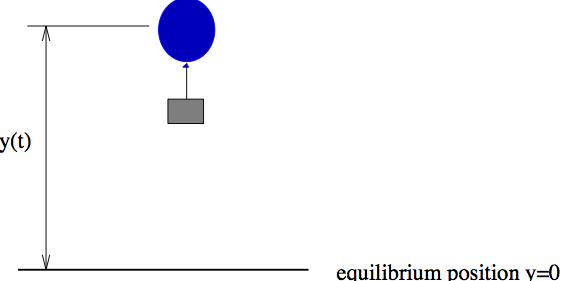
\includegraphics{balloon/balloon}
      \caption{A weather balloon oscillating about its level of
        neutral buoyancy.}
      \label{lab1:fig:balloon}
    \end{center}
  \end{figure}
\end{example}

\begin{problem}
  \label{lab1:prob:osc}
  \begin{itemize}
  \item a)
  Using the centered difference formula~\eqref{lab1:eq:centered-diff2}
  for the second derivative, and the forward difference
  formula~\eqref{lab1:eq:forward-diff} for the first derivative at the
  point $t_i$, derive a difference scheme for $y_{i+1}$, the vertical
  displacement of the weather balloon.
  
  \item b)
  What is the difference between this scheme and the forward
  Euler scheme from Example~\ref{lab1:exm:saturation}, related to the
  initial conditions?  (\textbf{Hint:} think about starting values \dots)
  
  \item c)
   Given the initial values above, explain how to start the numerical
  integration.

  \end{itemize}
\end{problem}

\subsection{Systems of First-order ODE's}
\label{lab1:sec:ode-system}

Discretization extends in a simple way to first-order systems of
ODE's, which arise in many problems, as we will see in some of the
later labs.  For now, though, we can see 

\begin{example}
  The second order DE for the weather balloon problem from
  Example~\ref{lab1:exm:balloon}
  can be rewritten by letting $u=dy/dt$.  Then,
  \[
    \frac{dy}{dt} = u 
  \]
  \[
    \frac{du}{dt} = -\frac{\beta}{m} u - \frac{\gamma}{m} y
  \]
  which is a system of first order ODE's in $u$ and $y$.  
  This set of differential equations can be discretized to obtain
  another numerical scheme for the weather balloon problem.
\end{example}

\begin{problem}
  \label{lab1:prob:osc-system}
  \begin{itemize}
  \item a)
  Derive a difference scheme for the problem based on the
  above system of two ODE's using the forward difference formula for
  the first derivative. 

  \item  b)
  By combining the discretized equations into  one  equation for y,
 show that the difference between this scheme and the scheme  obtained
 in problem one is the difference formula for the second derivative.
 
 \end {itemize}

\end{problem}


\subsection{Boundary Value Problems}
\label{lab1:sec:bvp}

So far, we've been dealing with \emph{initial value problems} or \emph{IVP's}
(such as 
the problem of heat conduction in a rock in
Example~\ref{lab1:exm:conduction}),
differential equation is given for an unknown function, along with its
initial value.  There is another class of problems, called {\em
  boundary value problems} (or \emph{BVP's}),  where the independent variables are
restricted to a \emph{closed domain} (as opposed to an \emph{open domain}) 
and the solution (or its
derivative) is specified at every point along the boundary of the
domain.  Contrast this to initial value problems, where the solution
is \emph{not given} at the end time.

A simple example of a boundary value problem is the steady
state heat diffusion equation problem for the rod in
Example~\ref{lab1:exm:diffusion1d}.  By \emph{steady state}, we mean
simply that the rod has reached a state where its temperature no
longer changes in time; that is, $\partial u/\partial t = 0$.  The
corresponding 
problem has a temperature, $u_(x)$, that depends on position only, and
obeys the following equation and boundary conditions:
\[ u_{xx} = 0, \]
\[ u(0) = u(1) = 0. \]
This problem is known as an \emph{initial-boundary value problem} (or
\emph{IBVP}), since it has a mix of both initial and boundary values. 

The structure of initial and boundary value problems are quite
different mathematically: IVP's involve a time variable which is
unknown at the end 
time of the integration (and hence the solution is known on an open
domain or interval), whereas BVP's specify the solution value on 
a closed domain or interval.  The 
numerical methods corresponding to these problems are also quite
different, and this can be best illustrated by an example.

\begin{example}
  \label{lab1:exm:steady-diffusion}
  We can discretize the steady state diffusion equation using the
  centered difference formula~\eqref{lab1:eq:centered-diff2} for the
  second derivative to obtain:
  \[
  u_{i+1}-2u_i+u_{i-1} = 0
  \]
  where $u_i\approx u(i/N)$ and $i=0,1,\ldots,N$ (and the factor of
  $(\Delta x)^2 = {1}/{N^2}$ has been multiplied out).  
  The boundary values $u_0$ and $u_N$ are both known to be zero, so
  the above expression represents a system of $N-1$ equations in $N-1$
  unknown values $u_i$ that must be solved for \emph{simultaneously}.
  The solution of such systems of linear equations will be covered in
  more detail in \htmladdnormallink{Lab~\#3}{\LabthreeURL} $-$ in
  fact, this equation forms the basis for a Problem in the
  Linear Algebra Lab~\externalref{lab3:sec:prob}.

  Compare this to the initial value problems discretized using the
  forward Euler method, where the resulting numerical scheme is
  a step-by-step, marching process (that is, the solution at one grid
  point can be computed using an explicit formula using only the value
  at the previous grid point).
\end{example}

\subsection{Partial Differential Equations}

So far, the examples of have been confined to ordinary differential
equations, but the procedure we've set out for ODE's extends with only
minor modifications to problems involving PDE's.  

\begin{example}
  To illustrate the process, let us go back to the heat diffusion
  problem from Example~\ref{lab1:exm:diffusion1d}, an initial-boundary
  value problem in the temperature $u(x,t)$:
  \[
  u_{t} = \alpha^2 u_{xx},
  \]
  along with initial values
  \[
  u(x,0) = u_0(x),
  \]
  and boundary values
  \[
  u(0,t) = u(1,t) = 0.
  \]
  
  As for ODE's, the steps in the process of discretization remain the
  same:
  \begin{enumerate}
  \item First, replace the independent variables by discrete values
    \[
    x_i = i \Delta x = \frac{i}{M}, \;\; \mbox{\rm where $i=0, 1,
      \ldots, M$, and}
    \]
    \[
    t_n = n \Delta t, \;\; \mbox{\rm where $n=0, 1,
      \ldots$}
    \]
    In this example, the set of discrete points define a two-dimensional
    grid of points, as pictured in Figure~\ref{lab1:fig:pde-grid}.
    \begin{figure}[htbp]
      \begin{center}
        \leavevmode
        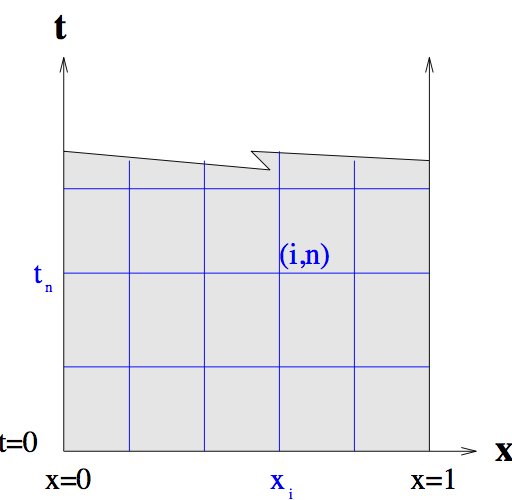
\includegraphics{pdes/pde-grid}
        \caption{The computational grid for the heat diffusion problem,
          with discrete points $(x_i,t_n)$.}
        \label{lab1:fig:pde-grid}
      \end{center}
    \end{figure}
    
  \item Replace the dependent variables (in this example, just the
    temperature $u(x,t)$) with approximations defined at the grid
    points:
    \[ 
    U_i^n \approx u(x_i,t_n).
    \]
    The boundary and initial values for the discrete temperatures can then
    be written in terms of the given information.
    
  \item Approximate all of the derivatives appearing in the problem with
    finite difference approximations.  
    If we use the centered difference
    approximation~\eqref{lab1:eq:centered-diff2} for the second
    derivative in $x$, and the forward difference
    formula~\eqref{lab1:eq:forward-diff} for the time derivative
    (while evaluating the terms on the right hand side at the previous
    time level), we obtain the following numerical scheme:
    \[
    U_i^{n+1} = U_i^n + \frac{\alpha^2 \Delta t}{(\Delta x)^2} \left(
      U_{i+1}^n - 2 U_i^n + U_{i-1}^n \right).
    \]
  \end{enumerate}
  Given the initial values, $U_i^0=u_0(x_i)$,
  and boundary values $U_0^n=U_M^n=0$, this difference formula allows
  us to compute values of temperature at any time, based on
  values at the previous time.

  There are, of course, other ways of discretizing this problem, but
  the above is one of the simplest.  
\end{example}


%%% Local Variables: 
%%% mode: latex
%%% TeX-master: "lab1"
%%% End: 
